\begin{surferIntroPage}{Tutorial}{tutorial_koord1}{צעדים ראשונים עם SURFER}
תוכנית זו נקראת SURFER. כאשר אתם קוראים את המילה, אתם ודאי חושבים על מים, שמש וגלים. אבל במקרה שלנו, שם התוכנית מבוסס על המילה האנגלית {\it surface} (משטח).
\\
עם SURFER ניתן להציג משטחים, או ליתר דיוק משטחים אלגבריים. מה פירוש הדבר ומה הם בעצם משטחים אלגבריים מוסבר להלן. כדי לעבור בין פרקי המדריך, פשוט לחצו על אחת התמונות (המשטחים) בצד ימין.\\
SURFER היא חלק מהתערוכה הנודדת IMAGINARY שהוצגה לראשונה במסגרת אירועי שנת המתמטיקה בגרמניה 2008. התערוכה היא פרוייקט של המוסד בעל המוניטין הבינלאומייםMathematisches Forschungsinstitut Oberwolfach (המכון למחקר מתמטי אובֶּרווֹלפַאך) הממוקם ביער השחור בגרמניה. בכל שבוע נערכות במכון סדנאות העוסקות בנושאים עכשוויים במחקר המתמטי. סדנאות אלה מעודדות חילופי ידע בין מדענים בכל רחבי העולם. \\
\vspace{0.2cm} \hspace{3.5cm}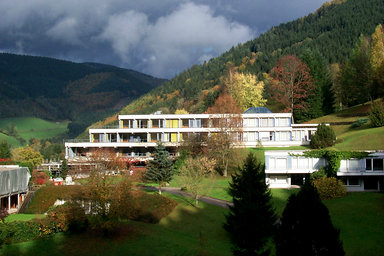
\includegraphics[width=3cm]{./../../common/images/photo_mfo.jpg}\\
ניתן להוריד את תוכנית SURFER בחינם מדף הבית שלנו: \\
\begin{centering}
www.imaginary.org\\
\end{centering}
 \vspace{0,2cm}
בצד ימין, תוכלו לבחור באחד מבין פרקי המדריך, החל במשטח ה-Zitrus. בצד שמאל, תוכלו לעבור לאחת מגלריות המשטחים בלחיצה על אחת התמונות או על הכיתוב שלידה.
\end{surferIntroPage}
